\chapter{Graphics Processing Units} \label{chapter:graphics_processing_units}

In this work, we aim to accelerate the execution of our solver using a relatively new architecture,
GPUs. GPUs are massively parallel computer chips that have recently started to be used in the
scientific computing domain. GPUs have initially been used to compute graphical computations, such
as the output to a computer screen, video processing, and synthetic image generation. These
computations are \textit{embarrassingly parallel}, meaning that they are comprised of many identical
computations independent of each other. GPUs are therefore optimised for parallel efficiency.
Combined with the fact that these problems deal with huge amounts of data, GPUs are also optimised
for maximum bandwidth. They are significantly different from \textit{Central Processing Units
(CPUs)}, the traditional architecture on which code is run. CPUs are optimised to solve serial
problems as fast as possible, meaning the prioritise serial speed over parallel efficiency, and
latency over bandwidth. 

Solving fluid flows over a mesh is a parallel problem, as at most steps it is possible to compute
the solution on the different elements making up the mesh in parallel. On the other hand, elements
must exchange information at their interfaces at each time step, meaning careful synchronisation
will be needed. Finally, the adaptivity process detailed in
Chapter~\ref{chapter:adaptive_mesh_refinement} and the load balancing process from
Chapter~\ref{chapter:load_balancing} are not inherently parallel processes. A lot of effort will
have put into breaking up these algorithms into parallel tasks to be run on GPUs. Overall, if it is
possible to efficiently parallelise these sequential parts of the problem, the gains from running
the main solving loop on the highly parallel GPUs should incur a significant speedup to the program.

\section{Architecture} \label{section:graphics_processing_units:architecture}
\subsection{Hardware model} \label{section:graphics_processing_units:architecture:hardware_model}

\begin{figure}[H]
	\centering
	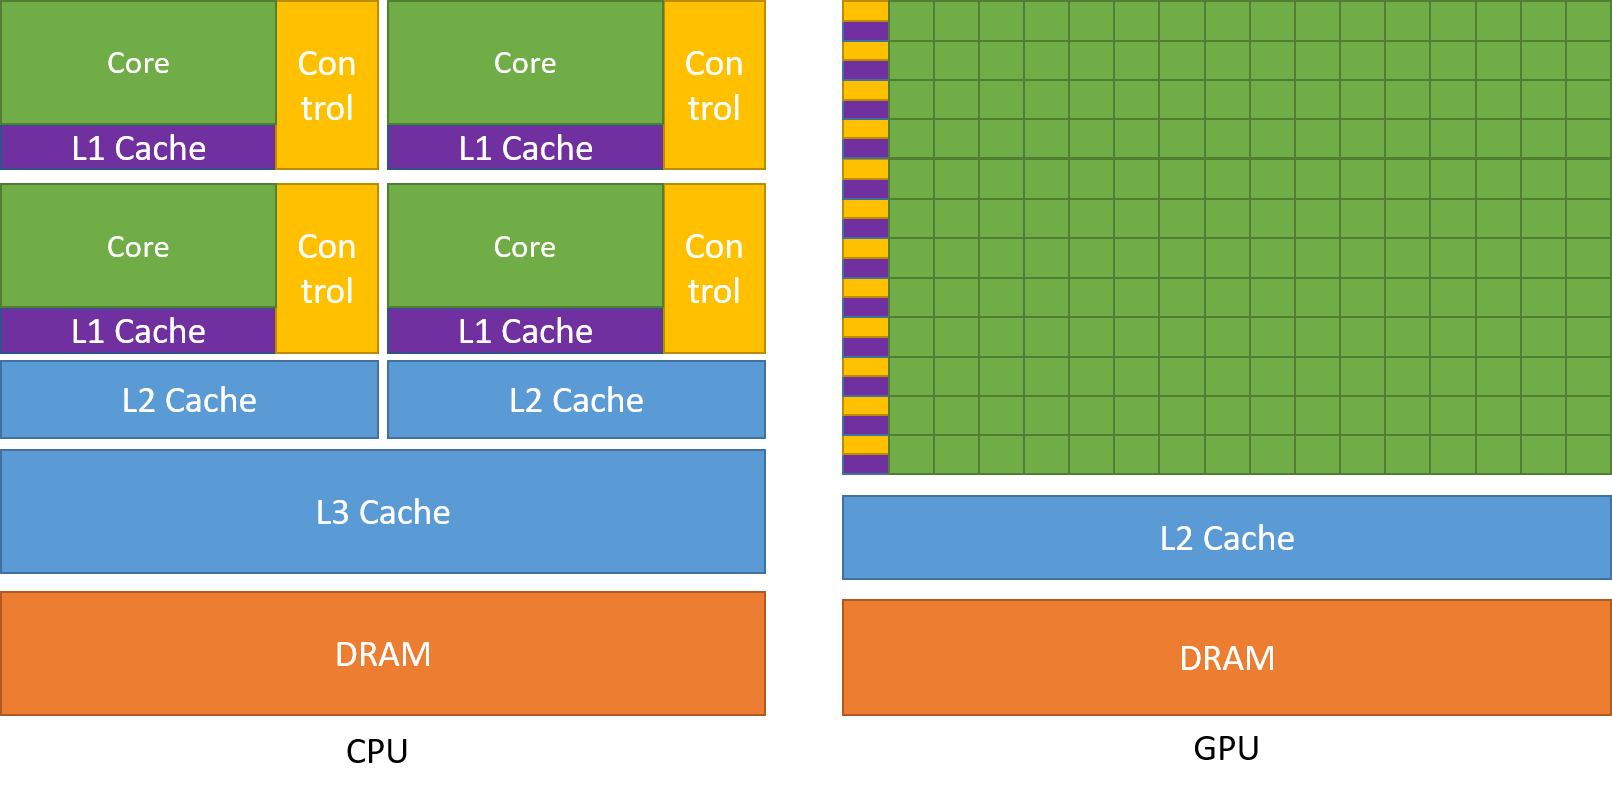
\includegraphics[width=0.8\textwidth]{Chapter_graphics_processing_units/media/gpu-devotes-more-transistors-to-data-processing}
	\caption{CPU and GPU architecture~\cite{Nvidia2021}: GPUs dedicate more space to data processing}
	\label{fig:cpu_gpu}
\end{figure}

Graphics processing units and central processing units are fundamentally made up of the same core
components. First, data processing hardware is shown in green. These are the parts of the chips that
do calculations on data. Then, in yellow is control flow. Control flow hardware schedules
instructions to be executed on processing hardware. In orange is the main memory of either
architecture. Main memory stores data to be used for computations. It is very big, and takes
relatively long to access. Finally, in blue and purple is different levels of cache. Cache is much
smaller and much faster than main memory, and as such stores parts of the memory that the processing
hardware is actively using in order to speed up access.

The two architectures differ as to the balance between the size and capacities of those components.
Chip area is limited by the processes used to manufacture them, so the different components must
share this limited spaces, and sacrifices must be made. GPUs dedicate much more space to data
processing, increasing throughput. Their compute units are also smaller, to work on more data in
parallel. CPUs, on the other hand, have fewer bigger compute units with a higher clock speed in
order to reduce latency. Their compute units are called cores. The GPU compute units are called CUDA
cores, and are arranged in rows as \textit{Streaming Multiprocessors (SMs)}.

In order to reduce latency, CPUs have a lot of die space dedicated to cache. More cache helps keep
data close in access time. More data is loaded from main memory at a time, assuming that data that
is near needed data will also be needed later. The deeper hierarchy of cache of CPUs helps keep the
cores working on the current as fast as possible, never starving for memory. GPUs have less total
cache and fewer levels of cache to make room for more CUDA cores. As a throughput oriented device,
it is less important how fast individual tasks complete, as long as more tasks overall are
completed. The reduced cache is acceptable because if a CUDA core is waiting on data from the main
memory that was not found in cache, it will simply pause execution of that thread and execute
another thread. On GPUs, the smallest and fastest cache, L1 cache, is shared within a SM. It is thus
fast to access shared data, as long as conflicts are avoided.

Finally, CPUs also reduce latency by using much more potent control flow units. Firstly, they have
one control flow unit per core, where GPUs have one control flow unit per row of cores. This limits
how many instruction can be dispatched to the cores making up a SM. The cores will therefore execute
the same execution at the same time in groups of 32, called warps. This makes branching much more
expensive if it happens within a warp. If a part of a program has two branches, A and B, the cores
executing branch A will execute, followed by the cores executing branch B. These have to be executed
sequentially because the control flow unit can only dispatch one instruction per warp. This
multiplies the computation time by the number of taken branches. CPU cores only execute a single
branch, or can even execute both branches at once while waiting for the result of the conditional,
keeping only the correct result once the conditional has been evaluated. The more powerful control
flow units of CPUs may also perform branch prediction, consisting of the CPU guessing the most
likely branch based on the result of previous computations and starting to execute this branch while
waiting for the conditional. All this is performed as an effort to reduce latency as much as
possible. Programs running on GPUs must compensate by avoiding divergence as much as possible within
warps.

\subsection{Programming model} \label{section:graphics_processing_units:architecture:programming_model}
% Talk about saturation, SMs
% How it doesn't work well with adaptivity usually

This work uses the CUDA programming model. It is a programming language, framework and runtime to
enable programming on GPUs with an extension of the C++ language. Programs using the language
execute on the CPU like a normal program, but can schedule parts of the program, called kernels, to
be executed on the GPU. Kernels are run in parallel on the GPU, asynchronously from the CPU. The CPU
is therefore free to do computations of its own while the GPU is executing, including adding more
kernels or transfers to the GPU execution queue. Multiple such queues, called streams, can exist.
The purpose of using multiple streams is to execute independent computations on the GPU
concurrently, and maximise GPU usage in case a stream is waiting. GPUs can concurrently execute
kernels, transfer data from the CPU to the GPU, and transfer data from the GPU to the CPU. These
transfers are necessary because CPU and GPU main random access memory are separate. This means that
data needed for computations on the GPU that cannot be generated on it must be explicitly
transferred from the CPU, and results living on the GPU must be transferred bact to the CPU in order
to be displayed or written to disk. As GPUs are also generally running the displays of non-server
computers, results that are only meant to be viewed can be directly displayed and skip such
transfers. This is not the case for this work.

\begin{figure}[H]
	\centering
	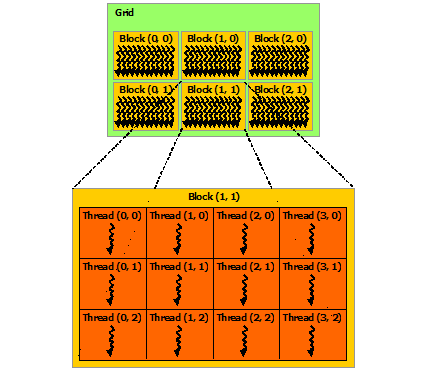
\includegraphics[width=0.6\textwidth]{Chapter_graphics_processing_units/media/grid-of-thread-blocks}
	\caption{GPU programming model~\cite{Nvidia2021}: Execution is split into multiple parallelism levels}
	\label{fig:gpu_programming_model}
\end{figure}

The programing model ties in with the hardware model from
subsection~\ref{section:graphics_processing_units:architecture:hardware_model} by decomposing the
execution of kernels to multiple parallel levels. A kernel will be executed in parallel, with each
core executing the same function. The whole problem to be solved it the grid. The kernel will
execute until the whole grid has been computed. The grid is broken up into blocks of threads. The
different blocks will be dispatched to the streaming multiprocessors of the GPU, and each thread of
that block will be executed on a CUDA core of the SM. A SM can execute multiple blocks at the same
time if there are more cores within the SM than threads within a block. Blocks need to be completely
independent of each other, as they cannot be synchronised and may execute in any order. They also
cannot share local memory, as each SM has its own L1 cache. Threads within the same block can depend
on one another, as they are executed concurrently on the same SM. Threads from a block execute the
same instruction at the same time in groups of 32, or warps. If there are more threads within a
block than cores within a SM, warps will be run sequentially until all threads are done with the
instruction. Threads within a block can share local memory, and synchronise with each other. This is
useful for algorithms with steps like reductions, where threads will wait until all threads have
computed one level of the reduction, to use the result of that level for the next one.

Typical execution of a program that adds an array A to an array B and stores the result in an array
C will go as following. The CPU side of the program will create two arrays of data in its memory,
and initialise them as needed. It will then create two arrays of the same size on the GPU using the
CUDA runtime, and transfer the data from the CPU arrays A and B to the GPU arrays. It will then
create a result array C on the GPU, and one on the CPU. It will then launch a kernel on the GPU, 
with pointers to the GPU A and B arrays, and the GPU C array. The number of elements in the vectors
will dictate the size of the execution grid. The number of elements will be split in blocks of
threads of fixed size, for example blocks of 128 threads. The number and size of blocks is given to
the GPU when calling the kernel. The CPU then must wait until the computation is done using a
synchronisation with the CUDA runtime, transfer the data from the GPU C array to the CPU C array,
and display the results. 

\section{Process Parallelism} \label{section:graphics_processing_units:process_parallelism}
% GPU partitions
% Say something about worker processes, to be general with cpu workers.

When trying to solve very large problems, a single node with a single GPU will have insufficient
processing power and memory to solve the problem in a reasonable time, or at all. To work with these
larger problems, the work needs to be split at another level than GPU parallelism.  

The program can use multi-block meshes, with each block being worked on by one process and one GPU.
If there are fewer GPUs available on a system than there are processes, some processes will share a
single GPU by using asynchronous execution streams. The different processes communicate together
using \textit{Message Passing Interface (MPI)} at their boundaries. Since the solution data resides
on the GPU, it must first be copied to the main CPU memory before it is sent through the MPI
runtime. It then needs to be copied to the receiving process' GPU. This exchange necessitates
multiple transfers on different levels and should be optimised as much as possible. An approach to
minimise the number of interfaces between the different mesh blocks is explained in
Chapter~\ref{chapter:load_balancing}. 

\section{Data structure} \label{section:graphics_processing_units:data_structure}
% Mesh design, unstructured
% Talk about dynamic memory
% Talk about data structure? The fact we use unstructured meshes, are the worse case for GPU
% Talk about how data is allocated
% Race conditions, when information is exchanged (ex fluxes)

\section{Implementation} \label{section:graphics_processing_units:implementation}
% Talk about reductions
% Talk about kernels
% Talk about reduce operations, data transfers for boundaries
